
\section{Thursday}\index{week3_Thursday_lecture}
\subsection{Announcement}
The assignment 2 requires to do a MATLAB project. The grade usually depends on your understanding of the reading materials and the time spent on experimentation.
\subsection{Sparse Large Scale Optimization}
Given an underlying signal $\bm x\in\mathbb{R}^n$ satisfying the undermined system $\bm{Ax}=\bm b$, we aim to recover the desired $\bm{\hat x}$. It suffices to solve the optimization problem
\[
\begin{array}{ll}
\min&\quad \|\bm D\bm x\|_1\\
\mbox{s.t.}&\quad\bm{Ax}= \bm b\\
&\bm A\in\mathbb{R}^{m\times n},m<n
\end{array}
\]
with $\bm D$ to be the difference matrix and $\min\|\bm{Dx}\|_1$ is sparsity promoting. Here we list two basic but effective ways to solve such a problem.

\paragraph{Linear Programming Approach}One way is to reformulate the problem into LP.
\begin{enumerate}
\item
Define new variables $t_i = |(\bm{Dx})_i|$, we can reformulate the origin problem as:
\[
\begin{array}{ll}
\min&\quad \sum_{i=1}^nt_i\\
\mbox{s.t.}&\quad\bm{Ax}= \bm b\\
&-t_i\le \sum_{k=1}^nd_{ik}x_k\le t_i\\
&\bm A\in\mathbb{R}^{m\times n},m<n
\end{array}
\]
\item
Alternatively, recall what we have learnt in MAT3007. Define slack variables $(\bm{Dx})_i = u_i -v_i $, where $u_i:=(\bm{Dx})_i^+, v_i =(\bm{Dx})_i^-$. It suffices to solve 
\[
\begin{array}{ll}
\min&\quad \sum_{i=1}^n(u_i+v_i)\\
\mbox{s.t.}&\quad\bm{Ax}= \bm b\\
&-t_i\le \sum_{k=1}^nd_{ik}x_k\le t_i\\
&\bm A\in\mathbb{R}^{m\times n},m<n\\
&u_i,v_i\ge0
\end{array}
\]
\end{enumerate}
However, linear programming is not the optimal way to solve large-scale problem.

\paragraph{Gredient-Based Approach}
We can also transform it into the unconstraint minimization problem, i.e., we add the penalty for the constraint $\bm{Ax} - \bm b=\bm0$:
\[
\min\|\bm D\bm x\|_1 + \frac{\mu}{2}\|\bm{Ax} - \bm b\|^2
\]
You may see that this reformulation is not exactly equivalent to the origin problem. However, it is not meaningful to stress $\bm{Ax}$ should exactly equal to $\bm b$, as there exsists some noise perturbing the equality in nature.

Another problem is that this objective function is not differentiable once there is at least zero entry from $\bm{Dx}$. Thus we do the approximation
\[
|t| \approx \sqrt{t^2+\sigma},\mbox{ for small }\sigma>0.
\]
Hence, it suffices to solve
\begin{equation}\label{Eq:3:1}
\min f(x):=\Theta_{\sigma}(\bm{Dx}) + \frac{\mu}{2}\|\bm{Ax} - \bm b\|^2
\end{equation}
where
\[
\Theta_{\sigma}(\bm y) = \sum_{i=1}^n\sqrt{y_i^2+\sigma}
\]

\paragraph{Descent Direction}
Since problem(\ref{Eq:3:1}) is convex, taking the derivative leads to minimum point. Hence we use the gredient descent method, i.e., $\bm d = -\nabla f(\bm x)$.

Although this direction is not optimal (trying another direction may be faster after several iterations), let's assume we are short-sighted such that we just want to take the steepest direction.

Hence the iterative algorithm to solve this problem can be summarized into one formula: Take a initial guess $\bm x^0$, then for $r=0,1,2\dots$
\[
\bm x^{r+1} = \bm x^r - \alpha^r\nabla f(\bm x^r)
\]
\paragraph{Stopping Criteria}
The stopping criteria has two conditions, either one is satisfied is ok. Always keep mind of scaling for stopping criteria, i.e., how large of an objective should depend on the scale of the problem.
\begin{itemize}
\item
First is $\|\nabla f(\bm x^k)\|\le 10^{-2}\|\nabla f(\bm x^0)\|$, i.e., the iterative method converge to the near stationary point
\item
Another is $|f(\bm x^k) - f(\bm x^{k+1})|\le 10^{-8}|f(\bm x^k)|$, i.e., the function does not change too much.
\end{itemize}

The next questions turn out that how to choose initial guess? How to choose step-length? Is steepest descent usuallt effective?
\begin{enumerate}
\item
For large-scale optimization, the steepest descent is usually one of the \emph{best} way among iterative methods.
\item
To choose the initial guess, sometimes we choose the LS solution, i.e., enter the matlab command $A'A/A'b$.
\item
Last lecture we tell that we can choose step-length to be the Lipstichz constant, but the disadvantage is that the constant $L$ for large scale optimization is too small. We have a better alternative.
\end{enumerate}

\paragraph{Armijo Condition and BB Step}The motivation is that we aim to let
\begin{equation}\label{Eq:3:2}
f(\bm x^k+\alpha\bm d^k)\le f(\bm x^k)+C_1\alpha \inp{\nabla f(\bm x)}{\bm d^k}, (0<C_1<1)
\end{equation}
i.e., our updated function value should be at least less than the old function minus the descent decrease gain, i.e., it should sufficiently decrease faster than a constant times the steepest gredient descent.

This method has a geometrically meaning:
\begin{figure}[H]
\centering
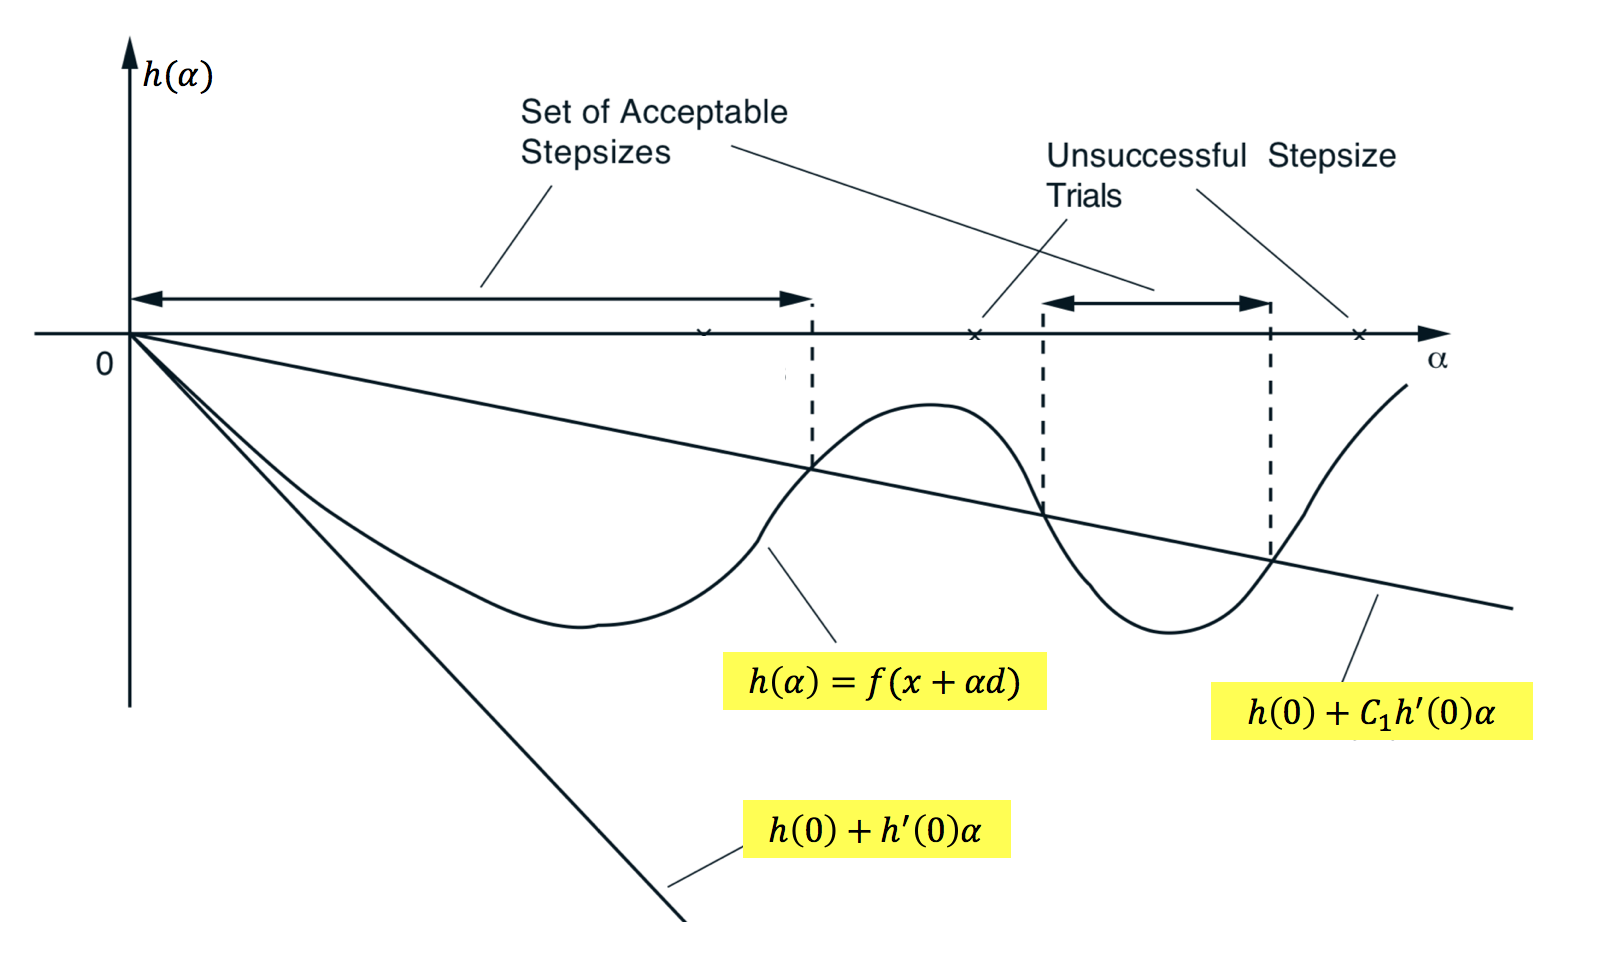
\includegraphics[width=15cm]{3_1.png}
\caption{Geometric Interpretaiton of Armijo Condition}
\end{figure}

We set $h(\alpha):=f(\bm x+\alpha\bm d)$, then $h'(0)=\inp{\nabla f(\bm x+\alpha\bm d)}{\bm d}$, thus the tangent line at $h(0)$ is given by:
\[
h(0)+\alpha h'(0):=f(\bm x)+\alpha\inp{\nabla f(\bm x+\alpha\bm d)}{\bm d}
\]

Geometrically we can see that no $\alpha$ can be chosen such that the updated function value $h(\alpha)$ is less than this tangent line. Hence we make the tangent line more flat, i.e., we want to find $\alpha$ such that the updated function value $h(\alpha)$ is below the line $h(0)+C_1h'(0)\alpha$, $0<C_1<1$:
\[
h(\alpha)\le h(0)+C_1h'(0)\alpha
\]

How to choose such $\alpha$? Take a initial long step-length $\bar{\alpha}$ first, if condition(\ref{Eq:3:2}) is not satisfied, try step length $\beta\bar{\alpha},\beta^2\bar{\alpha},\dots$ respectively. (Take a big step, if not satisfied, shorten the step.)
\begin{remark}
However, it is not sugested to do that. Although it is mathematically true, during the computer run, the step-length will decrease exponentially.
\end{remark}

How to choose $C_1$? Empirically, $C_1 = 10^{-3}$ or $10^{-4}$, i.e., it is very flat.

How to choose initial $\bar{\alpha}$? It depends on the scale of functionm which requires for your reading of materials.

How to choose the value of $\beta$? Do the experiment. (0.5, 0.8 for example).





